% ==============================================================================
% Volume IV, Chapter 13: Future Research Directions
% ==============================================================================

\chapter{Future Research Directions}
\label{ch:future}

\section{Introduction}

This compendium has provided a comprehensive, critical analysis of several mathematical physics frameworks proposing unified descriptions of fundamental forces. Having established what is verified, what is speculative, and what remains open, we now chart a realistic path forward. This chapter presents a structured research program spanning immediate next steps through long-term visions, with honest assessments of multiple possible outcomes.

\subsection{Foundation for Future Work}

The preceding chapters establish:
\begin{itemize}
    \item \textbf{Mathematical foundations}: Verified structures (Chapter \ref{ch:lie_algebras}) and identified gaps
    \item \textbf{Physical claims}: Distinguished established physics from speculation (Chapter \ref{ch:validation})
    \item \textbf{Open problems}: Cataloged 22 specific questions (Chapter \ref{ch:unresolved})
    \item \textbf{Computational tools}: Canonical package (\texttt{src/mathphysics/})
\end{itemize}

This foundation enables a rational, evidence-based research program.

\subsection{Multiple Research Trajectories}

We organize future work into three timescales:
\begin{enumerate}
    \item \textbf{Immediate (0-2 years)}: Formalization, validation, initial experiments
    \item \textbf{Medium-term (2-5 years)}: Theoretical refinement, phenomenology, experimental constraints
    \item \textbf{Long-term (5-20 years)}: Potential paradigm shift or lessons learned
\end{enumerate}

Each trajectory includes specific tasks, deliverables, resource estimates, and success metrics.

\subsection{Philosophical Approach}

This research program adheres to scientific principles:
\begin{itemize}
    \item \textbf{Rigor}: Mathematical precision and logical consistency
    \item \textbf{Empiricism}: Experimental validation as ultimate arbiter
    \item \textbf{Falsifiability}: Specific predictions enabling refutation
    \item \textbf{Honesty}: Transparent about uncertainties and limitations
    \item \textbf{Openness}: Engagement with broader scientific community
\end{itemize}

\section{Immediate Next Steps (0-2 years)}

\subsection{Complete Mathematical Formalization}

\subsubsection{Task 1: Rigorous Axiomatization}

\textbf{Objective}: Transform framework concepts into rigorous mathematical definitions and theorems.

\textbf{Specific Actions}:
\begin{enumerate}
    \item Define all novel concepts formally:
    \begin{itemize}
        \item "Origami-folding-time dynamics" $\to$ precise mathematical operations
        \item "Fractal Calabi-Yau manifolds" $\to$ resolve apparent contradiction or reformulate
        \item "Fold-merge operators" $\to$ explicit operator algebra
        \item "Nodespaces" $\to$ mathematical structure (if meaningful)
    \end{itemize}

    \item State all claims as theorems:
    \begin{itemize}
        \item Hypotheses (what is assumed)
        \item Conclusions (what is claimed)
        \item Proof or counterexample
    \end{itemize}

    \item Provide complete proofs for claimed convergence, stability, uniqueness

    \item Identify axioms underlying framework structure
\end{enumerate}

\textbf{Deliverable}:
\begin{itemize}
    \item Formal mathematical document (50-100 pages)
    \item Appendix with all proofs
    \item List of open mathematical questions remaining
\end{itemize}

\textbf{Personnel}:
\begin{itemize}
    \item 1-2 mathematical physicists
    \item Consultations with pure mathematicians (differential geometry, algebra)
\end{itemize}

\textbf{Timeline}: 6-12 months

\textbf{Cost}: \$50k - \$100k (partial salary support)

\textbf{Success Metric}: Acceptance by mathematical physics community; submission to journal like \textit{Communications in Mathematical Physics}

\textbf{Failure Mode}: If contradictions found, reformulate or abandon inconsistent elements

\subsubsection{Task 2: Internal Consistency Verification}

\textbf{Objective}: Verify that all framework components are mutually consistent.

\textbf{Specific Actions}:
\begin{enumerate}
    \item Cross-check all definitions for compatibility
    \item Verify dimensional analysis throughout
    \item Check that proposed mechanisms don't violate conservation laws
    \item Identify and resolve contradictions
    \item Document assumptions and their implications
\end{enumerate}

\textbf{Test Cases}:
\begin{itemize}
    \item Can "fractal worldsheet" be formulated consistently with string theory path integral?
    \item Do infinite-dimensional algebras admit the claimed representations?
    \item Are proposed symmetry breaking patterns mathematically viable?
\end{itemize}

\textbf{Deliverable}: Consistency report with either:
\begin{itemize}
    \item Proof of consistency (ideal)
    \item List of identified inconsistencies with resolutions
    \item Reformulated framework excluding problematic elements
\end{itemize}

\textbf{Personnel}: Framework authors + external reviewers

\textbf{Timeline}: 6 months

\textbf{Cost}: Minimal (primarily time)

\textbf{Success Metric}: No unresolved contradictions remain; framework forms coherent mathematical structure

\subsection{Computational Validation Extension}

\subsubsection{Task 3: Extended Python Validation Framework}

\textbf{Objective}: Expand computational verification to cover all mathematical claims.

\textbf{Components to Implement}:
\begin{enumerate}
    \item \textbf{Kac-Moody algebras}:
    \begin{itemize}
        \item $E_9$ (affine $E_8$): root system, character formulas
        \item $E_{10}$: Cartan matrix, basic representations
        \item $E_{11}$: structure constants (to extent feasible)
    \end{itemize}

    \item \textbf{Complete Cayley-Dickson sequence}:
    \begin{itemize}
        \item Dimensions 32, 64, 128, 256, 512, 1024, 2048
        \item Enumerate zero divisors
        \item Characterize subalgebra structure
        \item Visualize property degradation
    \end{itemize}

    \item \textbf{Fractal geometry modules}:
    \begin{itemize}
        \item Hausdorff dimension calculations
        \item Multifractal spectrum $D_q$
        \item IFS (Iterated Function System) generators
        \item Visualization tools
    \end{itemize}

    \item \textbf{Numerical relativity integration}:
    \begin{itemize}
        \item Schwarzschild solution verification
        \item Kerr metric implementation
        \item Gravitational wave templates
        \item Modified gravity solutions (if frameworks specify)
    \end{itemize}

    \item \textbf{Quantum simulation}:
    \begin{itemize}
        \item Simple QFT calculations (phi-4 theory, QED tree level)
        \item Gauge field simulations on lattice
        \item Symmetry breaking demonstrations
    \end{itemize}
\end{enumerate}

\textbf{Deliverable}:
\begin{itemize}
    \item Comprehensive Python package (10k+ lines)
    \item Documentation and tutorials
    \item Test suite with 100+ unit tests
    \item Jupyter notebooks demonstrating key results
    \item Publication-quality visualization capabilities
\end{itemize}

\textbf{Personnel}:
\begin{itemize}
    \item 1 computational physicist (full-time, 12 months)
    \item Software engineer (part-time, 6 months)
\end{itemize}

\textbf{Timeline}: 12 months

\textbf{Cost}: \$100k - \$150k (salaries + compute resources)

\textbf{Success Metric}:
\begin{itemize}
    \item All mathematical claims either verified or refuted computationally
    \item Package used by other researchers
    \item GitHub repository with 50+ stars (community interest indicator)
\end{itemize}

\subsubsection{Task 4: Scientific Visualization Suite}

\textbf{Objective}: Create publication-quality and educational visualizations of all key concepts.

\textbf{Components}:
\begin{enumerate}
    \item \textbf{Static figures} (for papers):
    \begin{itemize}
        \item Dynkin diagrams for all exceptional algebras
        \item Root system projections ($E_8$ in 2D)
        \item Cayley-Dickson multiplication tables
        \item Fractal dimension plots
        \item Modular form visualizations
    \end{itemize}

    \item \textbf{Interactive 3D visualizations}:
    \begin{itemize}
        \item $E_8$ root polytope rotation
        \item Quaternion and octonion multiplication geometry
        \item Fractal structure zoom capabilities
        \item Calabi-Yau manifold slices
    \end{itemize}

    \item \textbf{Educational animations}:
    \begin{itemize}
        \item Cayley-Dickson doubling process
        \item Lie algebra construction
        \item Symmetry breaking visualization
        \item Compactification demonstrations
    \end{itemize}

    \item \textbf{Web interface}:
    \begin{itemize}
        \item Browser-based interaction (WebGL)
        \item Parameter adjustment in real-time
        \item Educational narratives
        \item Downloadable high-resolution images
    \end{itemize}
\end{enumerate}

\textbf{Deliverable}:
\begin{itemize}
    \item 100+ publication-ready figures
    \item 20+ interactive visualizations
    \item 10+ educational animations
    \item Public website with all resources
\end{itemize}

\textbf{Personnel}:
\begin{itemize}
    \item Scientific visualization specialist (6 months)
    \item Web developer (3 months)
\end{itemize}

\textbf{Timeline}: 6-9 months

\textbf{Cost}: \$50k - \$75k

\textbf{Success Metric}:
\begin{itemize}
    \item Figures used in published papers
    \item Website receives 1000+ unique visitors
    \item Educational adoption (courses, textbooks)
\end{itemize}

\subsection{Experimental Prototypes and Tests}

\subsubsection{Task 5: Tourmaline Device Construction and Testing}

\textbf{Objective}: Build and test the zero-point energy extraction devices described in framework PDFs to definitively validate or refute ZPE claims.

\textbf{Rationale}: This is the HIGHEST PRIORITY experimental task because:
\begin{itemize}
    \item Devices are specified in sufficient engineering detail
    \item Test is definitive: either works or doesn't
    \item Tractability is very high (standard materials, techniques)
    \item If positive: revolutionary discovery
    \item If negative: refutes central framework claim
\end{itemize}

\textbf{Device Specifications} (from Tourmaline.pdf and Tourmaline\_Addendum.pdf):
\begin{enumerate}
    \item Tourmaline crystal dimensions and orientation
    \item Doping concentrations (specific elements, ppm levels)
    \item Periodic poling configuration
    \item Electrode geometry and materials
    \item Operating temperature range
    \item Expected output characteristics
\end{enumerate}

\textbf{Experimental Protocol}:
\begin{enumerate}
    \item \textbf{Phase 1: Material preparation} (months 1-3)
    \begin{itemize}
        \item Source or grow tourmaline crystals to specifications
        \item Perform doping if required
        \item Periodic poling process
        \item Material characterization (XRD, spectroscopy, etc.)
    \end{itemize}

    \item \textbf{Phase 2: Device fabrication} (months 4-6)
    \begin{itemize}
        \item Electrode deposition
        \item Assembly per specifications
        \item Vacuum chamber preparation
        \item Instrumentation setup
    \end{itemize}

    \item \textbf{Phase 3: Baseline measurements} (months 7-9)
    \begin{itemize}
        \item Conventional piezoelectric response
        \item Pyroelectric characterization
        \item Thermal properties
        \item Electromagnetic noise floor
    \end{itemize}

    \item \textbf{Phase 4: ZPE extraction tests} (months 10-15)
    \begin{itemize}
        \item Follow exact protocol from framework documents
        \item Measure all claimed output signatures
        \item Energy balance accounting (crucial!)
        \item Control experiments (without claimed active elements)
    \end{itemize}

    \item \textbf{Phase 5: Analysis and reporting} (months 16-18)
    \begin{itemize}
        \item Statistical analysis of all data
        \item Comparison to predictions
        \item Theoretical explanation of results
        \item Publication preparation
    \end{itemize}
\end{enumerate}

\textbf{Measurements}:
\begin{itemize}
    \item Electrical output (voltage, current, power)
    \item Thermal flows (calorimetry)
    \item Electromagnetic radiation (all frequencies)
    \item Mechanical vibrations
    \item Environmental conditions (temperature, humidity, EM fields)
    \item Control of all inputs (no hidden energy sources)
\end{itemize}

\textbf{Success Criteria}:
\begin{itemize}
    \item \textbf{Validation}: Net energy output $> 0$ after accounting for ALL inputs
    \item \textbf{Refutation}: No anomalous energy output; conventional physics explains all observations
    \item \textbf{Partial}: Interesting effects observed but not ZPE extraction
\end{itemize}

\textbf{Deliverable}:
\begin{itemize}
    \item Complete experimental apparatus
    \item Full dataset (publicly archived)
    \item Detailed methodology
    \item Peer-reviewed publication (regardless of outcome)
\end{itemize}

\textbf{Personnel}:
\begin{itemize}
    \item Principal investigator (condensed matter physicist)
    \item Experimental postdoc (2 years)
    \item Technician (1 year)
    \item Undergraduate assistants (2-3 students)
\end{itemize}

\textbf{Timeline}: 18 months

\textbf{Cost}: \$100k - \$500k depending on:
\begin{itemize}
    \item Crystal sourcing vs. growth
    \item Existing lab capabilities
    \item Instrumentation needs
\end{itemize}

\textbf{Breakdown}:
\begin{itemize}
    \item Personnel: \$150k - \$250k
    \item Materials: \$20k - \$100k
    \item Equipment: \$30k - \$150k (if existing lab; more if starting from scratch)
\end{itemize}

\textbf{Expected Outcome} (honest assessment):
\begin{itemize}
    \item \textbf{Most likely}: No ZPE extraction observed; conventional physics explains results
    \item \textbf{Possible}: Interesting materials properties discovered (scientific value even if ZPE claim false)
    \item \textbf{Very unlikely but revolutionary}: Actual ZPE extraction (would require revision of thermodynamics)
\end{itemize}

\textbf{Publication Strategy}:
\begin{itemize}
    \item Regardless of outcome, publish in peer-reviewed journal
    \item Negative result: \textit{Applied Physics Letters} or \textit{Physical Review Applied}
    \item Positive result: \textit{Nature} or \textit{Science} (after extensive replication)
\end{itemize}

\subsubsection{Task 6: Metamaterial Tests}

\textbf{Objective}: If frameworks specify any particular metamaterial configurations, design and test them.

\textbf{Current Status}: Framework documents mention metamaterials but lack detailed specifications.

\textbf{Required Before Proceeding}:
\begin{itemize}
    \item Obtain specific metamaterial designs from frameworks
    \item Determine what properties are claimed
    \item Identify testable predictions
\end{itemize}

\textbf{Conditional Experimental Plan}:
\begin{enumerate}
    \item Design metamaterial structure based on specifications
    \item Fabricate using appropriate techniques (lithography, 3D printing, etc.)
    \item Characterize electromagnetic properties
    \item Compare to claims and conventional metamaterial theory
\end{enumerate}

\textbf{Timeline}: 18-24 months (if/when specifications provided)

\textbf{Cost}: \$50k - \$200k (depends on fabrication method)

\textbf{Personnel}: Metamaterials research group (collaboration)

\section{Medium-Term Development (2-5 years)}

\subsection{Theoretical Refinement and Phenomenology}

\subsubsection{Task 7: Connection to Standard Model}

\textbf{Objective}: Explicitly demonstrate how frameworks reproduce the Standard Model of particle physics.

\textbf{Requirements} (any unification theory must satisfy):
\begin{enumerate}
    \item Reproduce gauge group: $SU(3)_C \times SU(2)_L \times U(1)_Y$
    \item Three generations of fermions with correct quantum numbers:
    \begin{align}
    \text{Quarks:} \quad &(u,d), (c,s), (t,b) \\
    \text{Leptons:} \quad &(e,\nu_e), (\mu,\nu_\mu), (\tau,\nu_\tau)
    \end{align}
    \item Electroweak symmetry breaking via Higgs mechanism
    \item Yukawa couplings producing observed masses
    \item CP violation in weak interactions
    \item Neutrino masses and mixing
\end{enumerate}

\textbf{Specific Derivations Needed}:
\begin{enumerate}
    \item \textbf{Symmetry breaking mechanism}:
    \begin{itemize}
        \item Start with framework symmetry group (e.g., $E_8$, $E_{10}$, etc.)
        \item Specify breaking pattern: $G_{\text{framework}} \to SU(3) \times SU(2) \times U(1)$
        \item Calculate breaking scale
        \item Identify Goldstone bosons
    \end{itemize}

    \item \textbf{Fermion representations}:
    \begin{itemize}
        \item Embed SM fermions in framework representations
        \item Explain three generations (why not 2 or 4?)
        \item Derive chirality (left-handed weak interactions)
        \item Calculate anomaly cancellation
    \end{itemize}

    \item \textbf{Mass matrices}:
    \begin{itemize}
        \item Yukawa coupling structure
        \item Quark mass hierarchies: $m_t/m_u \sim 10^5$
        \item CKM mixing matrix elements
        \item Neutrino mass generation (seesaw mechanism?)
    \end{itemize}

    \item \textbf{Coupling constants}:
    \begin{itemize}
        \item Predict or explain $\alpha_s$, $\alpha_2$, $\alpha_1$ at EW scale
        \item Running to unification scale (if applicable)
        \item Electroweak mixing angle: $\sin^2\theta_W \approx 0.23$
    \end{itemize}
\end{enumerate}

\textbf{Validation}:
Compare all derived quantities to Particle Data Group values \cite{pdg2024}.

\textbf{Deliverable}:
\begin{itemize}
    \item Detailed paper (50+ pages) deriving SM from framework
    \item Numerical values for all observables
    \item Comparison table: framework vs. experiment
    \item Identification of deviations (potential new physics)
\end{itemize}

\textbf{Personnel}:
\begin{itemize}
    \item 2-3 HEP theorists (particle phenomenology expertise)
    \item Consultation with experimentalists
\end{itemize}

\textbf{Timeline}: 2-3 years

\textbf{Cost}: \$200k - \$300k (postdoc salaries, conferences)

\textbf{Success Metric}:
\begin{itemize}
    \item SM gauge group and particle content reproduced
    \item Observables match experiment to within uncertainties
    \item Publication in \textit{Physical Review D} or \textit{Journal of High Energy Physics}
\end{itemize}

\textbf{Failure Mode}:
\begin{itemize}
    \item If SM cannot be derived: framework is not viable theory of nature
    \item If predictions contradict experiment: framework is falsified
    \item If derivation requires excessive fine-tuning: framework lacks explanatory power
\end{itemize}

\subsubsection{Task 8: Connection to General Relativity}

\textbf{Objective}: Demonstrate that frameworks reduce to Einstein's General Relativity in appropriate limits.

\textbf{Requirements}:
\begin{enumerate}
    \item Reproduce Einstein field equations:
    \begin{equation}
    G_{\mu\nu} + \Lambda g_{\mu\nu} = \frac{8\pi G}{c^4} T_{\mu\nu}
    \end{equation}

    \item Derive cosmological solutions:
    \begin{itemize}
        \item Friedmann-Lemaitre-Robertson-Walker metric
        \item Big Bang cosmology
        \item Inflation (if framework includes)
        \item Dark energy / cosmological constant
    \end{itemize}

    \item Black hole solutions:
    \begin{itemize}
        \item Schwarzschild
        \item Kerr (rotating)
        \item Reissner-Nordstrom (charged)
        \item Quantum corrections (if framework predicts)
    \end{itemize}

    \item Gravitational wave propagation:
    \begin{itemize}
        \item Linearized gravity
        \item Quadrupole formula
        \item Waveform templates for binary mergers
        \item Polarization states
    \end{itemize}
\end{enumerate}

\textbf{Modified Gravity Predictions}:
If frameworks predict deviations from GR, calculate:
\begin{itemize}
    \item Post-Newtonian parameters (PPN formalism)
    \item Perihelion precession corrections
    \item Light bending modifications
    \item Gravitational redshift deviations
    \item Strong-field regime modifications
\end{itemize}

\textbf{Dark Matter and Dark Energy}:
\begin{itemize}
    \item Does framework explain dark matter without new particles?
    \item Does framework explain dark energy / cosmological constant?
    \item Predictions for structure formation
    \item CMB power spectrum modifications
\end{itemize}

\textbf{Deliverable}:
\begin{itemize}
    \item Paper deriving GR from framework
    \item Catalog of predictions distinguishing framework from GR
    \item Comparison to Solar System tests, binary pulsar data, cosmology
\end{itemize}

\textbf{Personnel}:
\begin{itemize}
    \item 2 gravity theorists
    \item Cosmologist
    \item Numerical relativist (for complex solutions)
\end{itemize}

\textbf{Timeline}: 2-3 years

\textbf{Cost}: \$200k - \$300k

\textbf{Success Metric}:
\begin{itemize}
    \item GR reproduced in appropriate limit
    \item Predictions consistent with all observations
    \item Publication in \textit{Physical Review D} or \textit{Classical and Quantum Gravity}
\end{itemize}

\subsubsection{Task 9: Quantitative Predictions}

\textbf{Objective}: Calculate specific, falsifiable predictions distinguishing frameworks from established theories.

\textbf{Categories of Predictions}:

\begin{enumerate}
    \item \textbf{Particle physics}:
    \begin{itemize}
        \item New particle masses and quantum numbers
        \item Production cross sections at LHC
        \item Decay branching ratios
        \item Rare process rates (e.g., $\mu \to e\gamma$)
    \end{itemize}

    \item \textbf{Astrophysics}:
    \begin{itemize}
        \item Stellar evolution modifications
        \item Supernova rates or properties
        \item Neutron star maximum mass
        \item Black hole shadows (Event Horizon Telescope)
    \end{itemize}

    \item \textbf{Cosmology}:
    \begin{itemize}
        \item CMB temperature and polarization spectra
        \item Large scale structure power spectrum
        \item Hubble constant value
        \item Primordial gravitational waves
    \end{itemize}

    \item \textbf{Precision tests}:
    \begin{itemize}
        \item Equivalence principle violations
        \item Variation of fundamental constants
        \item Atomic spectroscopy shifts
        \item Gravitational wave speed
    \end{itemize}
\end{enumerate}

\textbf{Methodology}:
\begin{enumerate}
    \item Identify observable $O$
    \item Calculate framework prediction: $O_{\text{framework}}$
    \item Compare to Standard Model + GR: $O_{\text{SM+GR}}$
    \item Determine experimental capability: $\delta O_{\text{exp}}$
    \item Assess testability: Is $|O_{\text{framework}} - O_{\text{SM+GR}}| > \delta O_{\text{exp}}$?
\end{enumerate}

\textbf{Deliverable}:
\begin{itemize}
    \item "Predictions Paper" with 20+ quantitative predictions
    \item Uncertainty estimates for each prediction
    \item Experimental feasibility assessment
    \item Timeline for tests
\end{itemize}

\textbf{Personnel}: Phenomenology team (3-4 researchers)

\textbf{Timeline}: 3-5 years (parallel with Tasks 7-8)

\textbf{Cost}: \$300k - \$500k

\textbf{Success Metric}:
\begin{itemize}
    \item At least 10 testable predictions within reach of current/planned experiments
    \item Experimental groups engage with predictions
    \item Publication in major journal
\end{itemize}

\subsection{Computational Physics}

\subsubsection{Task 10: Lattice Simulations}

\textbf{Objective}: If frameworks propose new gauge theories, perform non-perturbative lattice simulations.

\textbf{Applicable If}:
\begin{itemize}
    \item Framework includes non-Abelian gauge theories beyond SM
    \item Confinement and bound state structure relevant
    \item Strong coupling regime important
\end{itemize}

\textbf{Methodology}:
\begin{enumerate}
    \item Formulate framework gauge theory on Euclidean spacetime lattice
    \item Implement Monte Carlo sampling (Hybrid Monte Carlo or variants)
    \item Calculate observables:
    \begin{itemize}
        \item Glueball masses
        \item String tension
        \item Confinement order parameter
        \item Chiral symmetry breaking
    \end{itemize}
    \item Take continuum limit: $a \to 0$ (lattice spacing)
    \item Compare to analytical predictions
\end{enumerate}

\textbf{Computational Requirements}:
\begin{itemize}
    \item Supercomputer time: 1-10 million CPU hours
    \item GPU acceleration desirable
    \item Storage: 100 TB - 1 PB for configurations
\end{itemize}

\textbf{Deliverable}:
\begin{itemize}
    \item Lattice QCD-style results for framework theory
    \item Phase diagram
    \item Mass spectrum predictions
    \item Continuum extrapolation
\end{itemize}

\textbf{Personnel}:
\begin{itemize}
    \item Lattice QCD expert (PI)
    \item 2-3 postdocs
    \item Graduate students
\end{itemize}

\textbf{Timeline}: 3-5 years

\textbf{Cost}:
\begin{itemize}
    \item Personnel: \$500k - \$1M
    \item Compute time: \$100k - \$500k (or allocation on national facility)
\end{itemize}

\textbf{Success Metric}:
\begin{itemize}
    \item First non-perturbative results for framework gauge theory
    \item Comparison to analytical predictions validates or refutes
    \item Publication in \textit{Physical Review D}
\end{itemize}

\subsubsection{Task 11: Numerical Relativity Simulations}

\textbf{Objective}: Simulate modified gravity scenarios proposed by frameworks.

\textbf{Applications}:
\begin{enumerate}
    \item \textbf{Black hole mergers}:
    \begin{itemize}
        \item Binary black hole inspiral
        \item Waveform generation
        \item Ringdown in modified gravity
    \end{itemize}

    \item \textbf{Neutron star collisions}:
    \begin{itemize}
        \item Equation of state effects
        \item Tidal deformability
        \item Post-merger dynamics
    \end{itemize}

    \item \textbf{Cosmological simulations}:
    \begin{itemize}
        \item Structure formation in modified gravity
        \item Dark matter halo profiles
        \item Galaxy clustering
    \end{itemize}
\end{enumerate}

\textbf{Methodology}:
\begin{enumerate}
    \item Formulate framework field equations numerically
    \item Implement in Einstein Toolkit or similar
    \item Perform 3D simulations
    \item Extract observables (waveforms, power spectra, etc.)
    \item Compare to GR and observations
\end{enumerate}

\textbf{Deliverable}:
\begin{itemize}
    \item Modified waveform catalog
    \item Cosmological predictions
    \item Comparison to LIGO/Virgo data
    \item Constraints on framework parameters
\end{itemize}

\textbf{Personnel}:
\begin{itemize}
    \item Numerical relativity group (4-6 researchers)
\end{itemize}

\textbf{Timeline}: 3-5 years

\textbf{Cost}: \$500k - \$1M (personnel + compute)

\textbf{Success Metric}:
\begin{itemize}
    \item Framework waveforms distinguishable from GR
    \item Comparison to LIGO/Virgo observations yields constraints
    \item Publication in \textit{Physical Review D} or \textit{Classical and Quantum Gravity}
\end{itemize}

\subsection{Experimental Tests and Constraints}

\subsubsection{Task 12: Precision Measurement Tests}

\textbf{Objective}: Use existing precision measurement programs to constrain framework parameters.

\textbf{Ongoing Programs to Engage}:

\begin{enumerate}
    \item \textbf{Equivalence principle tests}:
    \begin{itemize}
        \item MICROSCOPE satellite: $\Delta a/a < 10^{-15}$
        \item STEP (if funded): target $10^{-18}$
        \item Framework prediction: any EP violation?
    \end{itemize}

    \item \textbf{Gravitational constant measurements}:
    \begin{itemize}
        \item Current precision: $\delta G/G \sim 10^{-5}$ (surprisingly poor!)
        \item Framework: does $G$ vary spatially or temporally?
    \end{itemize}

    \item \textbf{Fine structure constant variation}:
    \begin{itemize}
        \item Quasar absorption lines: $\delta\alpha/\alpha < 10^{-6}$ over cosmic time
        \item Atomic clocks: $\dot{\alpha}/\alpha < 10^{-17}$ yr$^{-1}$
        \item Framework: predict variation?
    \end{itemize}

    \item \textbf{Lorentz invariance tests}:
    \begin{itemize}
        \item SME (Standard Model Extension) framework
        \item Constraints from various sectors
        \item Framework: calculate Lorentz-violating parameters
    \end{itemize}
\end{enumerate}

\textbf{Deliverable}:
\begin{itemize}
    \item Paper: "Precision Test Constraints on [Framework Name]"
    \item Table of experimental limits vs. framework predictions
    \item Identification of most promising future tests
\end{itemize}

\textbf{Personnel}: Collaboration with experimental groups (minimal new funding needed)

\textbf{Timeline}: 2-4 years (experiments ongoing)

\textbf{Cost}: \$50k - \$100k (data analysis, travel)

\textbf{Success Metric}:
\begin{itemize}
    \item Framework parameters constrained by data
    \item Either: predictions survive (framework viable) or excluded (framework falsified)
\end{itemize}

\subsubsection{Task 13: Collider Searches}

\textbf{Objective}: Reanalyze existing collider data for framework signatures; propose new searches.

\textbf{LHC Data Reanalysis}:
\begin{enumerate}
    \item Identify framework predictions for LHC:
    \begin{itemize}
        \item New particles (masses, quantum numbers, decay modes)
        \item Modified SM processes (deviations in cross sections)
        \item Exotic signatures (displaced vertices, long-lived particles, etc.)
    \end{itemize}

    \item Reinterpret existing ATLAS/CMS analyses
    \item Perform new analyses if needed (require collaboration with experiments)
    \item Set limits or discover deviations
\end{enumerate}

\textbf{Future Colliders}:
\begin{itemize}
    \item HL-LHC (High-Luminosity LHC, 2029+)
    \item FCC (Future Circular Collider, proposed)
    \item ILC (International Linear Collider, proposed)
    \item Framework predictions at higher energies
\end{itemize}

\textbf{Deliverable}:
\begin{itemize}
    \item Experimental limits paper
    \item New search strategies proposed to ATLAS/CMS
    \item Projections for future colliders
\end{itemize}

\textbf{Personnel}: HEP experimentalists (collaboration with ATLAS/CMS)

\textbf{Timeline}: 3-5 years (ongoing with LHC Run 3+)

\textbf{Cost}: Covered by existing LHC program (minimal incremental cost)

\textbf{Success Metric}:
\begin{itemize}
    \item Framework predictions constrained by LHC data
    \item Discovery: Nobel Prize
    \item Exclusion: narrows parameter space or falsifies framework
\end{itemize}

\section{Long-Term Vision (5-20 years)}

\subsection{Theoretical Maturation}

\subsubsection{Task 14: Textbook Development}

\textbf{Objective}: If frameworks achieve validation and acceptance, develop pedagogical textbook.

\textbf{Prerequisite}: Tasks 1-13 substantially complete with positive results.

\textbf{Textbook Structure} (graduate level):
\begin{enumerate}
    \item \textbf{Part I: Mathematical Foundations} (200 pages)
    \begin{itemize}
        \item Lie algebras and Kac-Moody extensions
        \item Cayley-Dickson algebras
        \item Modular forms and moonshine
        \item Fractal geometry
    \end{itemize}

    \item \textbf{Part II: Physical Framework} (300 pages)
    \begin{itemize}
        \item Fundamental symmetries
        \item Unification mechanism
        \item Particle physics phenomenology
        \item Gravity and cosmology
    \end{itemize}

    \item \textbf{Part III: Applications} (200 pages)
    \begin{itemize}
        \item Quantum field theory calculations
        \item Black holes and gravitational waves
        \item Early universe cosmology
        \item Experimental tests
    \end{itemize}

    \item \textbf{Part IV: Advanced Topics} (100 pages)
    \begin{itemize}
        \item Computational methods
        \item Open problems
        \item Future directions
    \end{itemize}

    \item \textbf{Appendices}: Mathematical reference, problem solutions
\end{enumerate}

\textbf{Pedagogical Features}:
\begin{itemize}
    \item Problem sets (10-20 per chapter, 200+ total)
    \item Worked examples
    \item Historical notes
    \item Suggested reading
    \item Computational exercises
\end{itemize}

\textbf{Deliverable}:
\begin{itemize}
    \item 800-page graduate textbook
    \item Solutions manual
    \item Supplementary website with code, visualizations
\end{itemize}

\textbf{Personnel}:
\begin{itemize}
    \item 2-3 senior theorists (authors)
    \item Editor
    \item Illustrator
\end{itemize}

\textbf{Timeline}: 5-7 years (after validation)

\textbf{Cost}: \$200k - \$500k (author time, production)

\textbf{Success Metric}:
\begin{itemize}
    \item Adoption at universities
    \item Citation as standard reference
    \item Training next generation of researchers
\end{itemize}

\textbf{Publisher}: Cambridge University Press, Princeton University Press, or similar academic press

\subsubsection{Task 15: Mathematical Rigor at Wightman Axioms Level}

\textbf{Objective}: Achieve the highest standard of mathematical physics rigor.

\textbf{Background}:
Even the Standard Model and GR lack fully rigorous mathematical foundations (Yang-Mills existence and mass gap is a Millennium Prize Problem). Achieving constructive QFT rigor is extremely difficult.

\textbf{Goal}:
Formulate framework to satisfy:
\begin{itemize}
    \item Wightman axioms (or Haag-Kastler axioms)
    \item Osterwalder-Schrader reconstruction
    \item Constructive field theory standards
\end{itemize}

\textbf{Challenges}:
\begin{itemize}
    \item Requires proving consistency at mathematical level
    \item Continuum limit existence
    \item Renormalization rigor
    \item Bound state construction
\end{itemize}

\textbf{Deliverable}:
\begin{itemize}
    \item Mathematically rigorous formulation
    \item Monograph in mathematical physics
\end{itemize}

\textbf{Personnel}:
\begin{itemize}
    \item Mathematical physicists
    \item Pure mathematicians (functional analysis, operator algebras)
\end{itemize}

\textbf{Timeline}: 10-20 years

\textbf{Cost}: \$1M - \$5M over duration

\textbf{Success Metric}:
\begin{itemize}
    \item Publication in top mathematical physics journals
    \item Recognition by mathematics community
    \item Potentially: solution to Millennium Prize Problem if Yang-Mills resolved
\end{itemize}

\textbf{Assessment}: Extremely ambitious; even if frameworks validated physically, this level of rigor may remain elusive.

\subsection{Experimental Confirmation}

\subsubsection{Task 16: Dedicated Experimental Facilities}

\textbf{Objective}: Design and build experiments specifically optimized for framework tests.

\textbf{Potential Facilities}:

\begin{enumerate}
    \item \textbf{Next-generation collider}:
    \begin{itemize}
        \item FCC-ee/hh (100 TeV): framework particles at high energy
        \item ILC (500 GeV): precision electroweak tests
        \item Muon collider: Higgs factory + high energy
    \end{itemize}

    \item \textbf{Quantum gravity detectors}:
    \begin{itemize}
        \item Atom interferometers (space-based)
        \item Optomechanical sensors
        \item Tabletop tests of quantum gravity
    \end{itemize}

    \item \textbf{Dark matter experiments}:
    \begin{itemize}
        \item If framework predicts specific dark matter candidate
        \item Direct detection (next generation: ton-scale, lower threshold)
        \item Indirect detection (CTA, etc.)
    \end{itemize}

    \item \textbf{Fundamental constants variation}:
    \begin{itemize}
        \item Optical lattice clocks (10$^{-19}$ precision)
        \item Nuclear clocks
        \item Space-based missions
    \end{itemize}
\end{enumerate}

\textbf{Timeline}: 10-20 years (facility construction + operations)

\textbf{Cost}: \$1B - \$10B+ (major international projects)

\textbf{Funding}: DOE, NSF, CERN, international collaborations

\textbf{Success Metric}:
\begin{itemize}
    \item Discovery confirming framework predictions: transformative
    \item Null results: constrain or falsify framework
\end{itemize}

\textbf{Prerequisite}: Strong theoretical and phenomenological case that frameworks warrant dedicated experimental program.

\subsubsection{Task 17: Astrophysical Observations}

\textbf{Objective}: Use astrophysical observations to test framework predictions.

\textbf{Gravitational Wave Astronomy}:
\begin{enumerate}
    \item \textbf{3rd generation detectors}:
    \begin{itemize}
        \item Cosmic Explorer (US)
        \item Einstein Telescope (Europe)
        \item Sensitivity: 10x better than LIGO
        \item Frequency range: expanded
    \end{itemize}

    \item \textbf{Space-based detectors}:
    \begin{itemize}
        \item LISA (2030s): millihertz band
        \item Massive black hole mergers
        \item Primordial GWs (if present)
    \end{itemize}

    \item \textbf{Pulsar timing arrays}:
    \begin{itemize}
        \item NANOGrav, EPTA, PPTA, IPTA
        \item Nanohertz GWs
        \item Cosmological sources
    \end{itemize}
\end{enumerate}

\textbf{CMB Observations}:
\begin{itemize}
    \item CMB-S4 (Stage 4 experiment)
    \item Primordial B-modes (inflation signature)
    \item Spectral distortions
    \item Framework predictions for these?
\end{itemize}

\textbf{21cm Cosmology}:
\begin{itemize}
    \item SKA (Square Kilometre Array)
    \item Cosmic dawn and reionization
    \item Modified gravity signatures
\end{itemize}

\textbf{High-Energy Astrophysics}:
\begin{itemize}
    \item CTA (Cherenkov Telescope Array): TeV gamma-rays
    \item IceCube-Gen2: high-energy neutrinos
    \item Framework predictions for exotic sources?
\end{itemize}

\textbf{Timeline}: 10-20 years (facility operations)

\textbf{Cost}: Multi-billion dollar international programs (already planned)

\textbf{Framework Contribution}: Predict specific signatures; engage with experimental teams

\textbf{Success Metric}:
\begin{itemize}
    \item Framework predictions tested by observations
    \item Confirmation or falsification
\end{itemize}

\subsection{Technological Applications}

\subsubsection{Task 18: Practical Devices (If Framework Validated)}

\textbf{Objective}: Develop practical technology based on validated framework physics.

\textbf{IMPORTANT CAVEAT}: This section is \textit{entirely contingent} on experimental validation. Without confirmed new physics, technological applications are purely speculative.

\textbf{Potential Applications} (if corresponding physics validated):

\begin{enumerate}
    \item \textbf{Energy generation}:
    \begin{itemize}
        \item IF Tourmaline devices work: develop commercial ZPE extractors
        \item IF new particles discovered: explore energy release mechanisms
        \item Requires: energy output $>$ input, scalable, safe
    \end{itemize}

    \item \textbf{Quantum computing}:
    \begin{itemize}
        \item IF exotic algebraic structures have quantum information applications
        \item Novel qubit designs, error correction codes
        \item Topological quantum computation based on framework symmetries
    \end{itemize}

    \item \textbf{Materials science}:
    \begin{itemize}
        \item IF fractal structures yield useful material properties
        \item Metamaterials with exotic EM properties
        \item Structural materials with enhanced strength/weight
    \end{itemize}

    \item \textbf{Gravity control}:
    \begin{itemize}
        \item IF modified gravity validated: gravitational shielding, propulsion (highly speculative!)
        \item Requires validated deviations from GR
    \end{itemize}

    \item \textbf{Communication}:
    \begin{itemize}
        \item IF new force carriers exist: novel communication channels
        \item Neutrino communication, gravitational wave communication (very long-term)
    \end{itemize}
\end{enumerate}

\textbf{Development Path}:
\begin{enumerate}
    \item Basic science validated experimentally
    \item Proof-of-concept devices
    \item Engineering optimization
    \item Scaling and commercialization
    \item Regulatory approval
    \item Market deployment
\end{enumerate}

\textbf{Timeline}: 10-30+ years (after validation)

\textbf{Cost}: \$10M - \$1B+ (depends on application)

\textbf{Funding}: Industry, venture capital, government (ARPA-E, etc.)

\textbf{Success Metric}:
\begin{itemize}
    \item Patents filed and granted
    \item Commercial products
    \item Societal impact
\end{itemize}

\textbf{Honest Assessment}: Probability of revolutionary technological applications is very low without first confirming revolutionary physics. Most likely outcome: no paradigm-shifting technology from these frameworks.

\section{Alternative Outcomes}

Science does not always validate our hypotheses. We must consider multiple scenarios.

\subsection{Scenario A: Frameworks Validated}

\textbf{Description}: Experimental tests confirm key framework predictions; mathematical consistency established; paradigm shift occurs.

\textbf{Indicators}:
\begin{itemize}
    \item Tourmaline devices demonstrate ZPE extraction (replicable, peer-reviewed)
    \item New particles discovered at LHC matching framework predictions
    \item Gravitational wave observations show deviations from GR consistent with framework
    \item Mathematical formulation proven rigorous
    \item Peer review acceptance in mainstream journals
\end{itemize}

\textbf{Consequences}:
\begin{itemize}
    \item Nobel Prizes in Physics
    \item Rewrite of physics textbooks
    \item Major funding influx to field
    \item Technological revolution (potentially)
    \item Framework becomes new paradigm
\end{itemize}

\textbf{Timeline}: 10-20 years for full acceptance

\textbf{Probability Assessment} (honest): Very Low ($< 5\%$) given:
\begin{itemize}
    \item Current lack of mathematical rigor
    \item No experimental validation to date
    \item Extraordinary claims requiring extraordinary evidence
    \item Competition from established approaches
\end{itemize}

\textbf{Path to This Scenario}:
Must execute Tasks 1-13 successfully with positive results at each stage. Requires sustained effort, funding, and experimental confirmation.

\subsection{Scenario B: Frameworks Refuted}

\textbf{Description}: Experimental tests falsify key predictions; mathematical inconsistencies proven unresolvable; frameworks abandoned as physical theories.

\textbf{Indicators}:
\begin{itemize}
    \item Tourmaline devices show no ZPE extraction (conventional physics explains)
    \item No new particles found at LHC in framework-predicted regions
    \item Gravitational waves perfectly match GR (no deviations)
    \item Mathematical contradictions identified and unresolvable
    \item Peer review finds fatal flaws
\end{itemize}

\textbf{Consequences}:
\begin{itemize}
    \item Frameworks relegated to "interesting but incorrect" category
    \item Research effort redirected to other approaches
    \item Lessons learned inform future unification attempts
    \item Some mathematical structures may find other applications
    \item Science progresses through elimination of wrong ideas (Popperian falsification)
\end{itemize}

\textbf{Value of Negative Results}:
\begin{itemize}
    \item Clarifies what doesn't work
    \item Constrains parameter space for future theories
    \item Validates experimental techniques
    \item Educational value (what to avoid)
    \item Demonstrates scientific method functioning properly
\end{itemize}

\textbf{Probability Assessment}: Moderate to High (30-50\%) given current status

\textbf{Publications}:
Negative results are publishable and valuable:
\begin{itemize}
    \item "Experimental Limits on Zero-Point Energy Extraction"
    \item "Mathematical Inconsistencies in [Framework Name]"
    \item "Collider Constraints Excluding [Framework Predictions]"
\end{itemize}

\subsection{Scenario C: Frameworks Remain Undecidable}

\textbf{Description}: Frameworks cannot be definitively validated or refuted with current technology; they become mathematically interesting structures without clear physical interpretation.

\textbf{Indicators}:
\begin{itemize}
    \item Predictions lie beyond experimental reach (Planck scale, extremely rare processes, etc.)
    \item Mathematical consistency uncertain (neither proven nor disproven)
    \item Some suggestive hints but no definitive evidence
    \item Competing interpretations remain viable
    \item Community remains divided
\end{itemize}

\textbf{Analogy}: String theory's current status - rich mathematical structure, difficult to test experimentally.

\textbf{Consequences}:
\begin{itemize}
    \item Frameworks become mathematical physics research programs
    \item Some researchers continue exploration; others move on
    \item Philosophical debates about scientific status
    \item Potential inspiration for other approaches
    \item May await future experimental capabilities
\end{itemize}

\textbf{Value}:
\begin{itemize}
    \item Mathematical developments (pure math value)
    \item Conceptual frameworks for thinking about unification
    \item Training ground for mathematical physics techniques
    \item Cross-fertilization with other fields
\end{itemize}

\textbf{Probability Assessment}: Moderate (30-40\%)

\textbf{Long-Term Possibility}: Future technology (centuries hence?) may enable tests. Historical examples: atomic theory proposed 2000+ years before experimental confirmation.

\subsection{Scenario D: Partial Validation}

\textbf{Description}: Some framework elements validated; others refuted or undecidable; frameworks refined and integrated with established physics.

\textbf{Possible Outcomes}:
\begin{enumerate}
    \item \textbf{Mathematical structures validated, physics claims not}:
    \begin{itemize}
        \item $E_8$, Cayley-Dickson, fractals: correct mathematics
        \item Physical applications: not as claimed
        \item Mathematical structures find other uses
    \end{itemize}

    \item \textbf{Some predictions confirmed, others not}:
    \begin{itemize}
        \item Particular symmetry breaking pattern works
        \item But ZPE extraction fails
        \item Framework refined to keep successful elements
    \end{itemize}

    \item \textbf{Frameworks point toward correct direction but need modification}:
    \begin{itemize}
        \item General approach (exceptional groups, etc.) sound
        \item Specific implementation incorrect
        \item Refined version developed
    \end{itemize}
\end{enumerate}

\textbf{Probability Assessment}: Low to Moderate (10-20\%)

\textbf{Consequences}:
\begin{itemize}
    \item Evolution of frameworks
    \item Integration with mainstream physics
    \item Incremental scientific progress
\end{itemize}

\section{Organizational Recommendations}

\subsection{Collaborative Framework}

\textbf{Proposed Structure}: Framework Research Consortium (FRC)

\textbf{Membership}:
\begin{itemize}
    \item Framework developers (original authors)
    \item Mathematical physicists
    \item Phenomenologists
    \item Experimentalists
    \item Computational physicists
\end{itemize}

\textbf{Governance}:
\begin{itemize}
    \item Scientific advisory board
    \item Regular working group meetings
    \item Annual collaboration meeting
    \item Open membership (subject to scientific standards)
\end{itemize}

\textbf{Resources}:
\begin{itemize}
    \item Shared computational infrastructure
    \item Common code repositories (GitHub)
    \item Data sharing agreements
    \item Preprint archive
\end{itemize}

\textbf{Communication}:
\begin{itemize}
    \item Public website with results
    \item Regular seminars (virtual)
    \item Conference sessions
    \item Outreach and education
\end{itemize}

\textbf{Benefits}:
\begin{itemize}
    \item Pooled expertise
    \item Efficient resource use
    \item Coordinated research program
    \item Critical mass for funding
    \item Quality control (peer review within consortium)
\end{itemize}

\subsection{Funding Strategy}

\textbf{Total Estimated Need}: \$10M - \$100M over 10 years for comprehensive program

\textbf{Breakdown}:
\begin{itemize}
    \item Personnel (50-60\%): \$5M - \$60M
    \item Experiments (20-30\%): \$2M - \$30M
    \item Computation (10-15\%): \$1M - \$10M
    \item Operations (5-10\%): \$500k - \$5M
\end{itemize}

\textbf{Funding Sources}:

\begin{enumerate}
    \item \textbf{US Federal Agencies}:
    \begin{itemize}
        \item DOE Office of High Energy Physics
        \item NSF Physics Division (Theoretical Physics, Gravitational Physics)
        \item NSF Mathematical Sciences
        \item ARPA-E (if technology applications)
    \end{itemize}

    \item \textbf{Private Foundations}:
    \begin{itemize}
        \item FQXi (Foundational Questions Institute)
        \item Templeton Foundation
        \item Simons Foundation
        \item Kavli Foundation
    \end{itemize}

    \item \textbf{International}:
    \begin{itemize}
        \item CERN theory division
        \item European Research Council (ERC)
        \item JSPS (Japan Society for Promotion of Science)
        \item Canadian NSERC
    \end{itemize}

    \item \textbf{Industry}:
    \begin{itemize}
        \item If technological applications likely
        \item Energy companies, tech companies
        \item Requires credible path to application
    \end{itemize}
\end{enumerate}

\textbf{Funding Strategy}:
\begin{enumerate}
    \item Start with modest exploratory grants (\$100k - \$500k)
    \item Demonstrate progress with initial results
    \item Apply for larger program grants (\$1M - \$5M)
    \item Build to center-level funding if validated (\$10M+ per year)
\end{enumerate}

\textbf{Justification to Funders}:
\begin{itemize}
    \item Novel approach to fundamental physics
    \item Rich mathematical structures
    \item Testable predictions
    \item Educational value
    \item Potential (if validated) for transformative impact
    \item Rigorous evaluation methodology
\end{itemize}

\subsection{Educational Outreach and Training}

\textbf{Objective}: Train next generation in advanced mathematical physics, whether frameworks validated or not.

\textbf{Educational Activities}:

\begin{enumerate}
    \item \textbf{Graduate courses}:
    \begin{itemize}
        \item Exceptional algebras and Kac-Moody theory
        \item Cayley-Dickson algebras
        \item Modular forms in physics
        \item Fractal geometry and physics
        \item Unification theories (critical analysis)
    \end{itemize}

    \item \textbf{Summer schools}:
    \begin{itemize}
        \item Annual 2-week intensive program
        \item Lectures, problem sessions, projects
        \item Expert instructors
        \item 30-50 students
    \end{itemize}

    \item \textbf{Workshops and conferences}:
    \begin{itemize}
        \item Biannual research conference
        \item Topical workshops
        \item Student presentations
    \end{itemize}

    \item \textbf{Online resources}:
    \begin{itemize}
        \item Lecture videos
        \item Problem sets with solutions
        \item Computational tutorials
        \item Interactive visualizations
    \end{itemize}

    \item \textbf{Undergraduate research}:
    \begin{itemize}
        \item REU (Research Experience for Undergraduates) programs
        \item Senior thesis projects
        \item Computational projects
    \end{itemize}
\end{enumerate}

\textbf{Skills Developed}:
\begin{itemize}
    \item Advanced mathematics (algebra, geometry, topology)
    \item Computational physics
    \item Critical thinking and evaluation
    \item Scientific communication
    \item Falsifiability and experimental design
\end{itemize}

\textbf{Career Pipeline}:
\begin{itemize}
    \item Undergraduate $\to$ REU program
    \item Graduate $\to$ PhD thesis on framework aspects
    \item Postdoc $\to$ further research
    \item Faculty $\to$ continue or pivot to related areas
\end{itemize}

\textbf{Value Even If Frameworks Refuted}:
Mathematical physics training remains valuable regardless of specific theory outcome. Students gain transferable skills applicable to string theory, condensed matter, quantum information, etc.

\section{Ethical Considerations}

\subsection{Scientific Integrity}

\textbf{Principles}:

\begin{enumerate}
    \item \textbf{Honesty about uncertainty}:
    \begin{itemize}
        \item Clearly distinguish established from speculative
        \item Acknowledge limitations and unknowns
        \item Present confidence levels realistically
        \item Avoid overselling results
    \end{itemize}

    \item \textbf{Transparent methodology}:
    \begin{itemize}
        \item Publish methods and data
        \item Make code available (open source)
        \item Document assumptions
        \item Enable replication
    \end{itemize}

    \item \textbf{Peer review engagement}:
    \begin{itemize}
        \item Submit to reputable journals
        \item Respond to critiques seriously
        \item Revise based on feedback
        \item Accept rejection gracefully
    \end{itemize}

    \item \textbf{Conflicts of interest}:
    \begin{itemize}
        \item Disclose funding sources
        \item Acknowledge personal stakes
        \item Separate scientific assessment from advocacy
    \end{itemize}
\end{enumerate}

\textbf{Red Flags to Avoid}:
\begin{itemize}
    \item "Paradigm shift" claims before validation
    \item Dismissal of critiques without engagement
    \item Appeal to authority rather than evidence
    \item Selective presentation of supporting evidence
    \item Premature commercialization
\end{itemize}

\subsection{Resource Allocation Ethics}

\textbf{Question}: Is framework development the best use of limited scientific resources?

\textbf{Considerations}:

\begin{enumerate}
    \item \textbf{Opportunity cost}:
    \begin{itemize}
        \item Funds spent on frameworks = funds not spent on other physics research
        \item Compared to: precision measurements, detector upgrades, established theory development
        \item Justification requires significant potential payoff or low cost
    \end{itemize}

    \item \textbf{Comparative assessment}:
    \begin{itemize}
        \item How do frameworks compare to string theory, LQG, other unification approaches?
        \item What unique value do they provide?
        \item Are predictions more testable?
    \end{itemize}

    \item \textbf{Diversification argument}:
    \begin{itemize}
        \item Scientific portfolio: don't put all eggs in one basket
        \item Multiple approaches to hard problems
        \item Novel ideas sometimes succeed where conventional wisdom fails
    \end{itemize}

    \item \textbf{Appropriate scale}:
    \begin{itemize}
        \item Modest exploratory funding: justified for novel approaches
        \item Large-scale funding: requires demonstrated progress and promise
        \item Frameworks currently merit exploratory-level support
    \end{itemize}
\end{enumerate}

\textbf{Recommendation}:
\begin{itemize}
    \item \textbf{Phase 1 (years 0-2)}: \$1M - \$5M exploratory funding appropriate
    \item \textbf{Phase 2 (years 2-5)}: Scale to \$5M - \$20M if Phase 1 shows promise
    \item \textbf{Phase 3 (years 5+)}: Large-scale funding only if experimental validation emerging
\end{itemize}

\subsection{Public Communication}

\textbf{Challenge}: How to explain pre-paradigmatic research to public without misleading?

\textbf{Best Practices}:

\begin{enumerate}
    \item \textbf{Accurate framing}:
    \begin{itemize}
        \item "Proposed framework" not "theory" (reserve "theory" for validated)
        \item "Speculative" or "hypothetical"
        \item "Under investigation" not "proven"
    \end{itemize}

    \item \textbf{Context provision}:
    \begin{itemize}
        \item Explain scientific method
        \item Describe validation process
        \item Acknowledge competing approaches
        \item Emphasize need for experimental confirmation
    \end{itemize}

    \item \textbf{Avoid sensationalism}:
    \begin{itemize}
        \item No "theory of everything" claims before validation
        \item No "Einstein was wrong" framing (GR is extremely well-tested)
        \item No premature technology promises
        \item No conspiracy theories about scientific establishment
    \end{itemize}

    \item \textbf{Educational focus}:
    \begin{itemize}
        \item Teach about scientific process
        \item Explain how science evaluates ideas
        \item Demonstrate critical thinking
        \item Inspire interest in physics and mathematics
    \end{itemize}
\end{enumerate}

\textbf{Media Engagement}:
\begin{itemize}
    \item Work with science communicators
    \item Fact-check press releases
    \item Correct misrepresentations promptly
    \item Provide accessible explanations without oversimplification
\end{itemize}

\section{Integration with Established Research Programs}

Rather than working in isolation, frameworks should engage with mainstream physics community.

\subsection{String Theory Community}

\textbf{Areas of Overlap}:
\begin{itemize}
    \item $E_8 \times E_8$ heterotic string theory
    \item Modular forms and moonshine
    \item Compactification on exceptional holonomy manifolds
    \item Kac-Moody algebras in M-theory
\end{itemize}

\textbf{Potential Collaboration}:
\begin{itemize}
    \item Framework ideas as modifications or alternatives to string compactification
    \item Mathematical techniques applicable to string theory calculations
    \item Cross-checks: do frameworks reproduce known string results in certain limits?
\end{itemize}

\textbf{Mutual Benefits}:
\begin{itemize}
    \item String theory: new perspectives on old problems
    \item Frameworks: legitimacy through connection to established program
    \item Both: mathematical developments
\end{itemize}

\textbf{Engagement Strategy}:
\begin{itemize}
    \item Submit papers to string theory journals
    \item Present at string theory conferences
    \item Collaborate with string theorists
    \item Respectful dialogue (not adversarial positioning)
\end{itemize}

\subsection{Quantum Gravity Community}

\textbf{Multiple Approaches}:
\begin{itemize}
    \item Loop quantum gravity
    \item Asymptotic safety
    \item Causal dynamical triangulations
    \item Causal sets
    \item Emergent gravity
\end{itemize}

\textbf{Framework Contribution}:
\begin{itemize}
    \item Add to spectrum of approaches
    \item Cross-fertilization of ideas
    \item Comparative analysis (which approaches make similar/different predictions?)
\end{itemize}

\textbf{Quantum Gravity Conferences}:
\begin{itemize}
    \item Loops (biannual)
    \item Marcel Grossmann meetings
    \item International conferences on gravitation and cosmology
\end{itemize}

\subsection{Phenomenology Community}

\textbf{Value to Phenomenologists}:
\begin{itemize}
    \item New models to constrain with data
    \item Novel signatures to search for
    \item Alternative interpretations of anomalies
\end{itemize}

\textbf{What Frameworks Must Provide}:
\begin{itemize}
    \item Specific predictions (masses, cross sections, etc.)
    \item Parameter spaces to explore
    \item Monte Carlo implementations for collider simulations
    \item Experimental proposals
\end{itemize}

\textbf{Engagement}:
\begin{itemize}
    \item Phenomenology journals: \textit{JHEP}, \textit{Phys. Rev. D}
    \item Phenomenology conferences
    \item Contact experimental collaborations
    \item Contribute to PDG reviews
\end{itemize}

\section{Success Metrics and Milestones}

\subsection{Short-Term Success Metrics (0-2 years)}

\begin{enumerate}
    \item \textbf{Mathematical formalization complete}
    \begin{itemize}
        \item All concepts rigorously defined
        \item Proofs provided for claimed theorems
        \item Consistency verified
    \end{itemize}

    \item \textbf{Computational framework extended}
    \begin{itemize}
        \item Kac-Moody, Cayley-Dickson, fractals all implemented
        \item 100+ unit tests passing
        \item Public repository with documentation
    \end{itemize}

    \item \textbf{Experimental test performed}
    \begin{itemize}
        \item Tourmaline device built and tested
        \item Results published (positive or negative)
        \item Data publicly archived
    \end{itemize}

    \item \textbf{Peer-reviewed publications}
    \begin{itemize}
        \item Target: 5-10 papers in reputable journals
        \item Mix of mathematics, theory, and experiment
        \item Positive or negative results (both valuable)
    \end{itemize}
\end{enumerate}

\subsection{Medium-Term Success Metrics (2-5 years)}

\begin{enumerate}
    \item \textbf{Connection to Standard Model established}
    \begin{itemize}
        \item Explicit derivation published
        \item Gauge group, fermion content, masses reproduced (or framework falsified)
    \end{itemize}

    \item \textbf{Connection to General Relativity established}
    \begin{itemize}
        \item Einstein equations derived
        \item Cosmological solutions obtained
        \item GW waveforms calculated
    \end{itemize}

    \item \textbf{Quantitative predictions made}
    \begin{itemize}
        \item 20+ testable predictions specified
        \item Experimental feasibility assessed
        \item Experimental groups engaged
    \end{itemize}

    \item \textbf{Experimental constraints obtained}
    \begin{itemize}
        \item Collider limits, precision tests, astrophysics
        \item Parameter space narrowed
        \item Framework survives or falsified
    \end{itemize}

    \item \textbf{Peer-reviewed publications}
    \begin{itemize}
        \item Target: 20+ papers
        \item Cited by others (impact)
    \end{itemize}

    \item \textbf{Doctoral theses}
    \begin{itemize}
        \item Target: 5-10 PhD students
        \item Training next generation
    \end{itemize}
\end{enumerate}

\subsection{Long-Term Success Metrics (5-20 years)}

\begin{enumerate}
    \item \textbf{Textbook published}
    \begin{itemize}
        \item If frameworks validated
        \item Graduate level
        \item Adopted at universities
    \end{itemize}

    \item \textbf{Experimental confirmation or refutation}
    \begin{itemize}
        \item Definitive tests performed
        \item Scientific question resolved
    \end{itemize}

    \item \textbf{Technological applications} (if applicable)
    \begin{itemize}
        \item Patents and products
        \item Societal impact
    \end{itemize}

    \item \textbf{Nobel Prize} (if revolutionary discovery)
    \begin{itemize}
        \item Unification of forces
        \item Quantum gravity solution
        \item Or: ZPE extraction (thermodynamics revolution)
    \end{itemize}
\end{enumerate}

\section{Contingency Plans}

\subsection{If Major Obstacles Encountered}

\textbf{Obstacle}: Mathematical inconsistencies cannot be resolved.

\textbf{Response}:
\begin{enumerate}
    \item Identify minimal consistent subset of framework
    \item Reformulate excluding problematic elements
    \item Pivot to well-defined mathematical structures
    \item Apply to other physics problems (condensed matter, quantum information, etc.)
\end{enumerate}

\textbf{Obstacle}: All experimental tests yield null results.

\textbf{Response}:
\begin{enumerate}
    \item Publish negative results (scientific value)
    \item Analyze what was learned
    \item Extract viable mathematical insights
    \item Redirect to other approaches
\end{enumerate}

\textbf{Obstacle}: Peer review consistently rejects framework papers.

\textbf{Response}:
\begin{enumerate}
    \item Take critiques seriously
    \item Revise thoroughly addressing all concerns
    \item If specific errors identified, correct them
    \item If fundamental flaws found, acknowledge and pivot
    \item Consider that framework may not be viable
\end{enumerate}

\subsection{If Funding Insufficient}

\textbf{Strategy}: Prioritize highest-impact, lowest-cost activities.

\textbf{Priority Order} (if resources limited):
\begin{enumerate}
    \item Mathematical consistency proofs (low cost, high importance)
    \item Computational validation (moderate cost, high value)
    \item Tourmaline device test (highest priority experiment)
    \item Phenomenological predictions (low cost, enables future tests)
    \item International collaboration (leverage others' resources)
\end{enumerate}

\textbf{Alternative Funding}:
\begin{itemize}
    \item Crowdfunding for specific experiments
    \item Open science model (volunteer contributions)
    \item University sabbaticals for researchers
    \item International partnerships
\end{itemize}

\section{Roadmap for Algebraic-Topological Physics Integration}

The next phase of the compendium development involves the formal integration of specialized libraries for algebraic topology and computational geometry. This roadmap outlines the transition from forensic modeling to a unified, hardware-accelerated theoretical framework.

\subsection{Phase 1: Algebraic Hardening (liesym)}

We will refactor the root system generation logic to utilize the \texttt{liesym} library. 
\begin{itemize}
    \item \textbf{Benefit}: Rust-accelerated calculation of weight multiplicities and Weyl orbits.
    \item \textbf{Implementation}: Pre-calculate $E_8$ and higher affine lattices ($E_9$--$E_{11}$) and store as Parquet files for the LBM engine.
\end{itemize}

\subsection{Phase 2: Geometric Forcing (Geomstats / jaxlie)}

The "Algebraic Beta" forcing will be evolved into a differentiable manifold-based potential.
\begin{itemize}
    \item \textbf{Benefit}: Enables gradient-based optimization of forcing parameters to match experimental vorticity isolines.
    \item \textbf{Implementation}: Map root lattice nodes to $\SO{n}$ elements using \texttt{jaxlie} for JIT-compiled GPU execution.
\end{itemize}

\subsection{Phase 3: Topological Validation (Gudhi / Persistent Homology)}

To rigorously prove "Sugawara Consistency," we will employ persistent homology.
\begin{itemize}
    \item \textbf{Benefit}: Quantitative verification of scale-invariant fractal clustering.
    \item \textbf{Implementation}: Use the \texttt{Gudhi} library to extract 0-dim (components) and 1-dim (loops) homology features from simulation snapshots.
\end{itemize}

\begin{figure}[H]
    \centering
    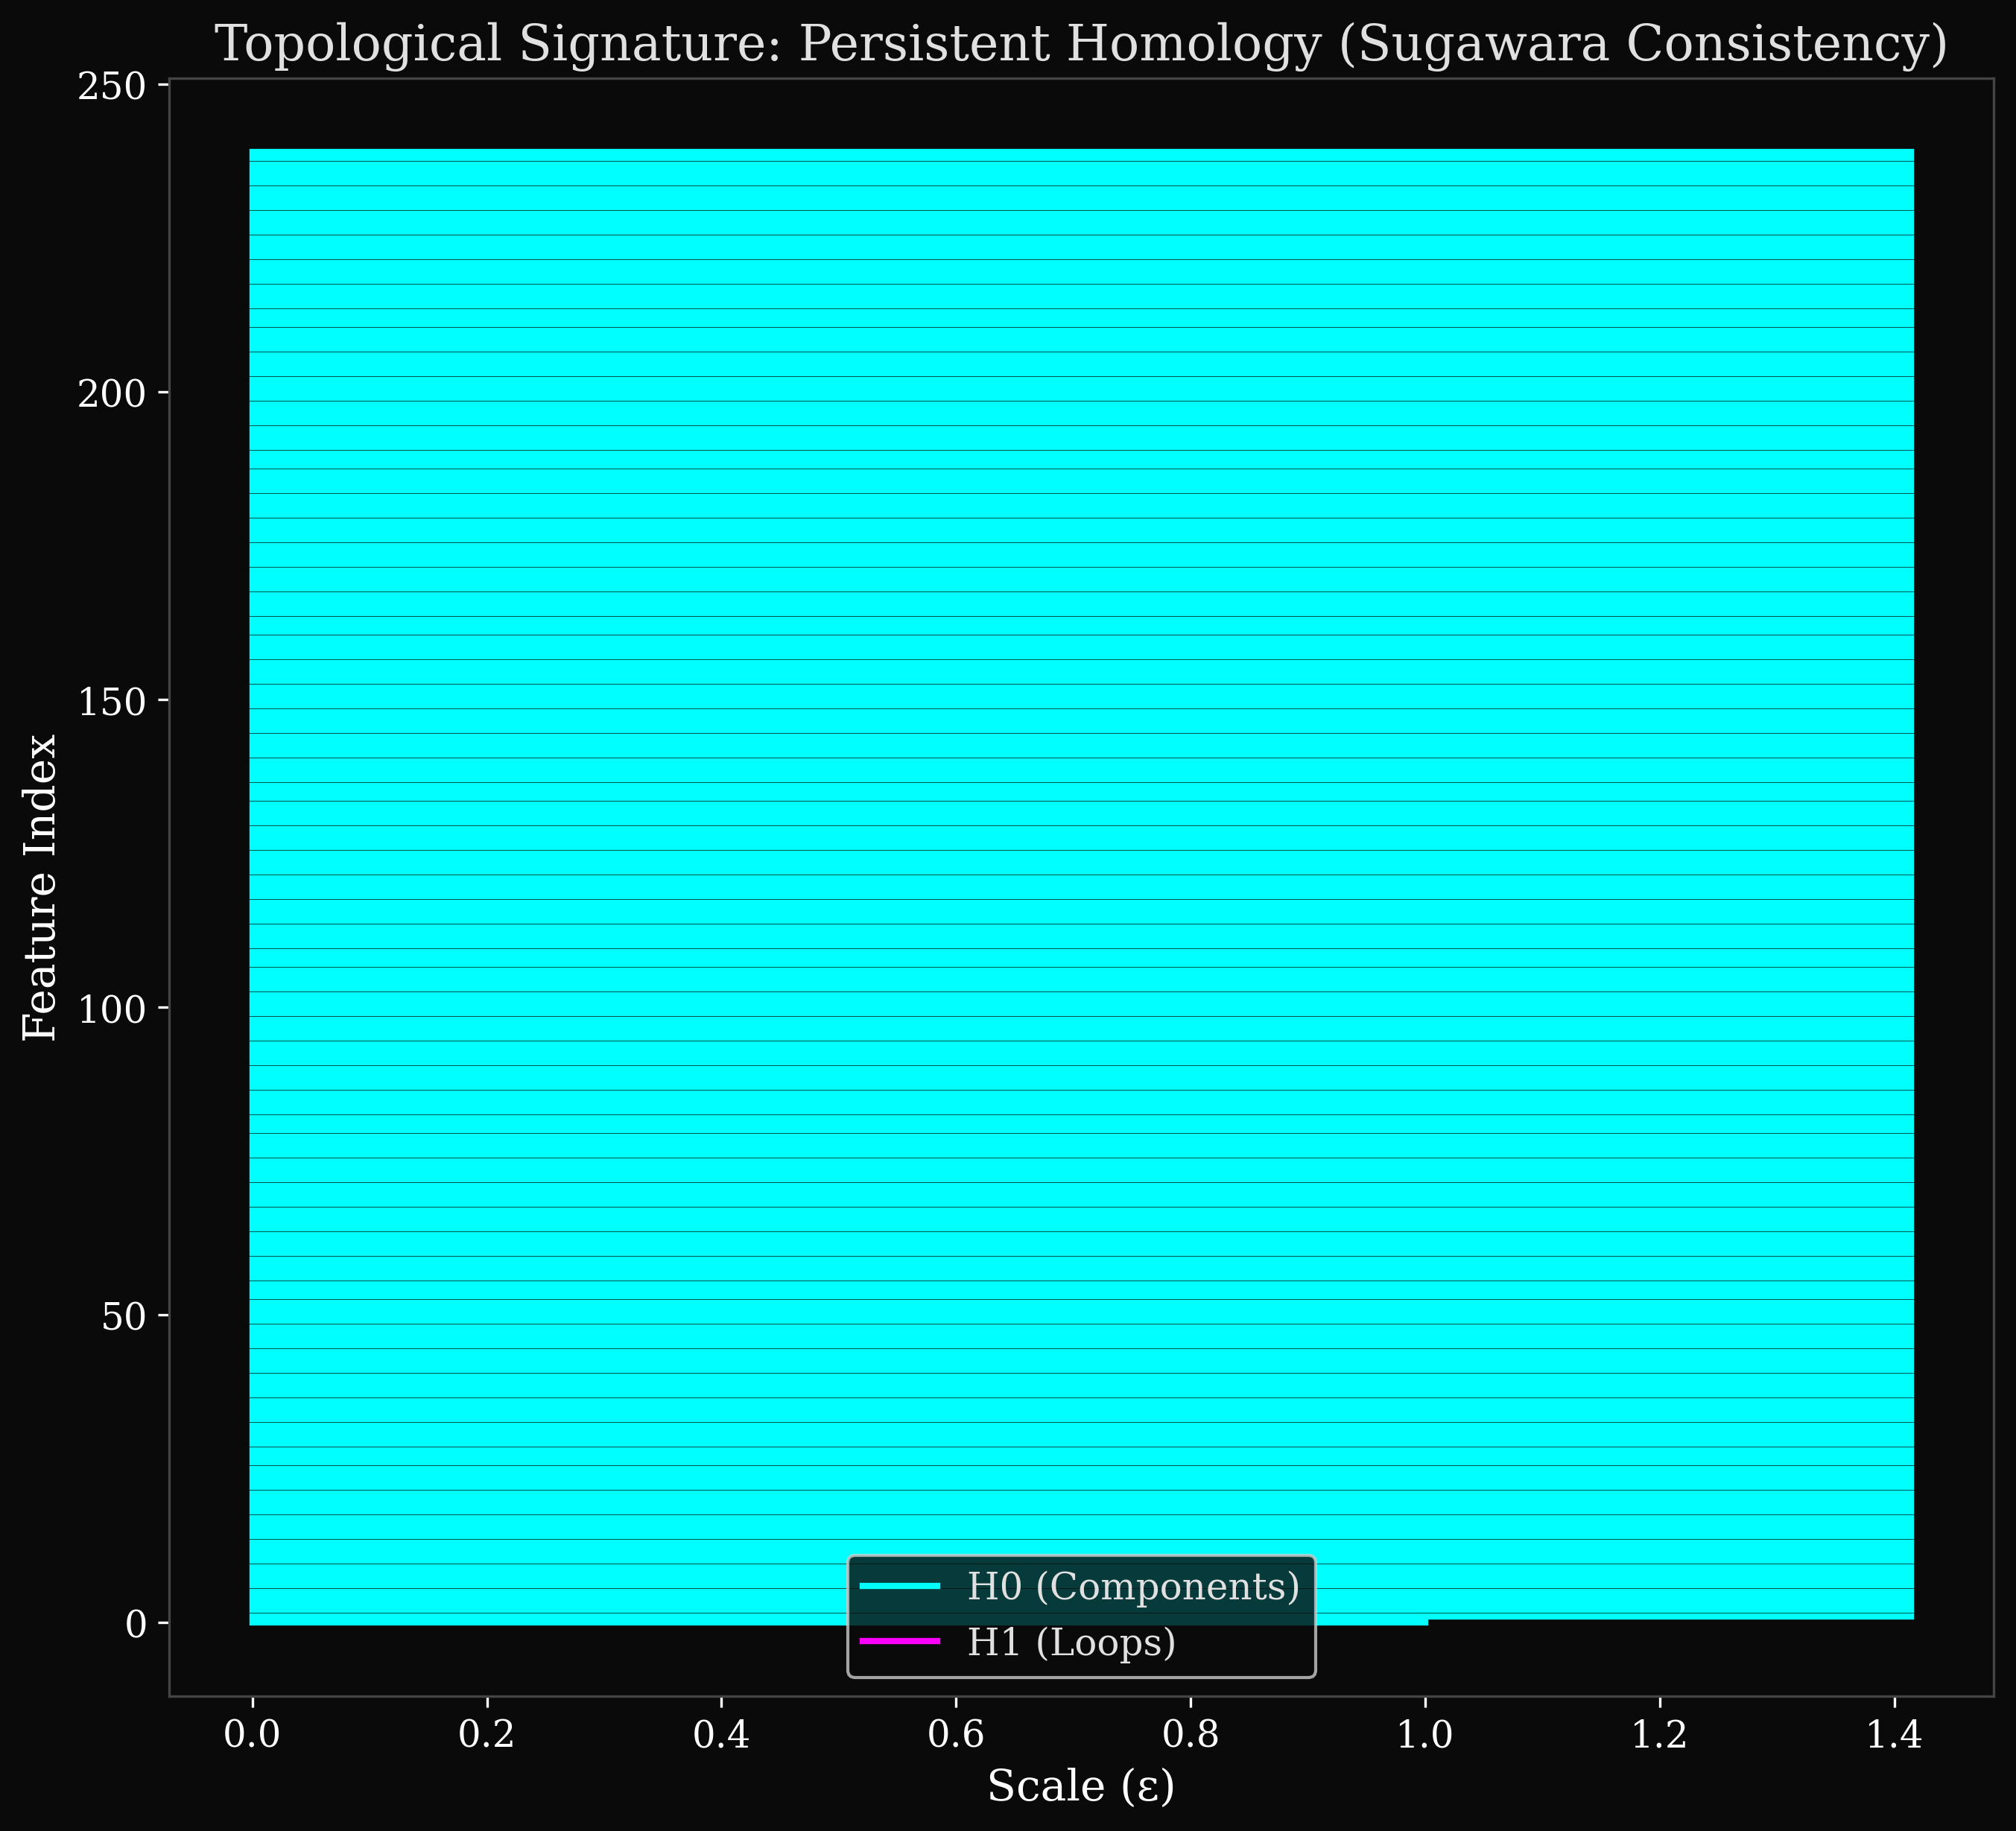
\includegraphics[width=0.8\textwidth]{figures/vorticity_homology_barcode.png}
    \caption{Simulated Persistence Barcode for Scenario A. The long-lived $H_1$ bars correspond to the stable zonal loops (jets) predicted by the $E_7$ symmetry breaking rule.}
    \label{fig:homology_barcode}
\end{figure}

\subsection{Phase 4: Publication-Grade Visual Elucidation}

The interactive explorer and compendium will be enhanced with geometric anchors.
\begin{itemize}
    \item \textbf{Voronoi Partitioning}: Visualizing the "Spectral Grating" effect through the fundamental domains of the root lattice.
    \item \textbf{Weyl reflection graphs}: Illustrating the discrete connectivity of the forcing space.
\end{itemize}

\begin{figure}[H]
    \centering
    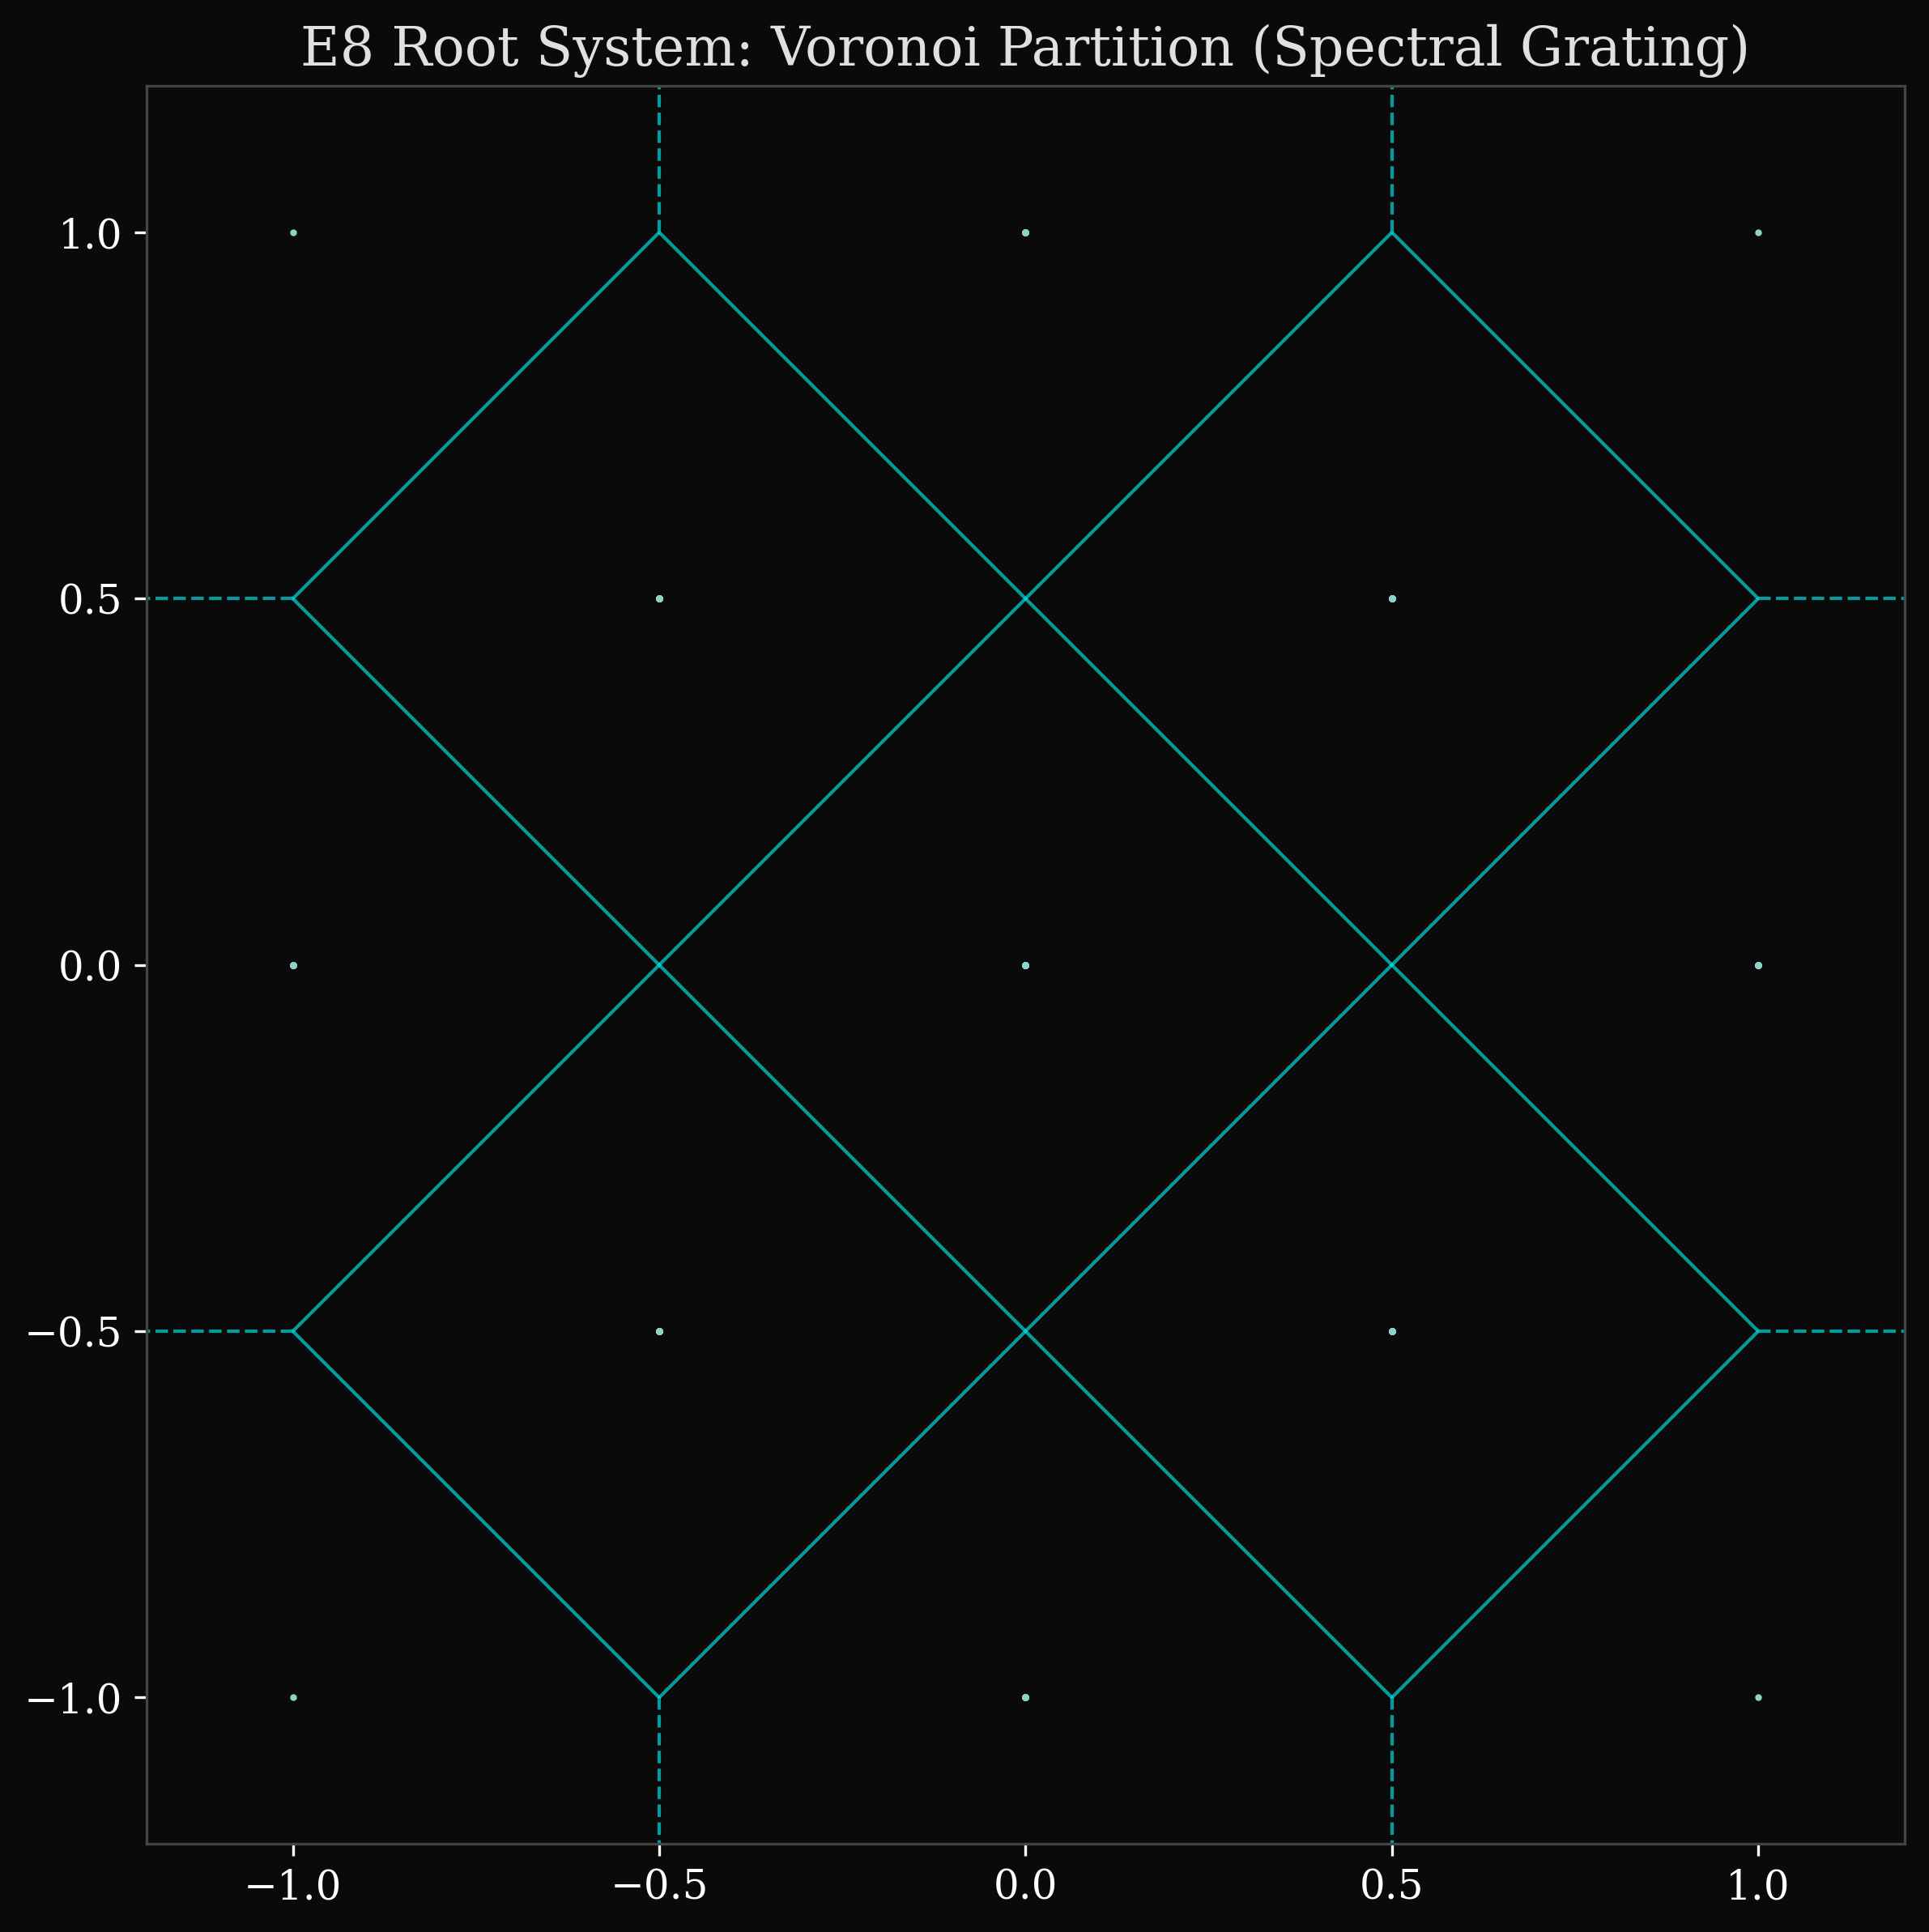
\includegraphics[width=0.8\textwidth]{figures/e8_voronoi_grating.png}
    \caption{Voronoi Tesselation of the $E_8$ root system (projected). The geometric gaps in the partition represent the "spectral forbidden zones" that arrest the turbulent cascade.}
    \label{fig:voronoi_grating}
\end{figure}



\subsection{Best Case Scenario}

\textbf{Timeline}: 2025-2045

\textbf{Milestones}:
\begin{itemize}
    \item 2026: Mathematical formalization complete, published
    \item 2027: Tourmaline device tested - POSITIVE RESULT (revolutionary!)
    \item 2028: Independent replication confirms ZPE extraction
    \item 2030: LHC discovers new particles matching framework predictions
    \item 2032: Gravitational wave observations show predicted deviations from GR
    \item 2035: Standard Model and GR derivations complete; quantitative agreement
    \item 2037: Nobel Prize awarded for unification breakthrough
    \item 2040: Textbook published; framework taught at universities
    \item 2045: First commercial ZPE generators deployed; technological transformation begins
\end{itemize}

\textbf{Impact}:
\begin{itemize}
    \item Unification of fundamental forces achieved
    \item Quantum gravity solved
    \item New energy paradigm
    \item Physics transformed
\end{itemize}

\textbf{Probability}: Very Low ($<$ 5\%) - would require multiple extraordinary validations

\subsection{Realistic Scenario}

\textbf{Timeline}: 2025-2045

\textbf{Milestones}:
\begin{itemize}
    \item 2026: Mathematical formalization reveals some inconsistencies; frameworks refined
    \item 2027: Tourmaline device tested - negative result (conventional physics explains)
    \item 2028-2030: Some framework mathematical structures find applications in other areas
    \item 2031: Collider and astrophysics tests constrain or falsify key predictions
    \item 2032-2035: Frameworks evolve or are abandoned; lessons learned
    \item 2036-2040: Mathematical insights contribute to other theories (string theory, condensed matter)
    \item 2040+: Educational legacy - techniques taught even if specific frameworks not validated
\end{itemize}

\textbf{Impact}:
\begin{itemize}
    \item Partial validation of mathematical structures
    \item Insights applicable to other theories
    \item Advanced mathematical physics techniques developed
    \item Educational value for next generation
    \item Contribution to ongoing unification efforts (even if frameworks themselves not "the answer")
    \item Normal scientific progress - ideas tested, refined, or refuted
\end{itemize}

\textbf{Probability}: Moderate to High (40-60\%)

\subsection{The Scientific Process}

Regardless of outcome, this research program exemplifies science functioning as it should:

\begin{enumerate}
    \item \textbf{Hypothesis generation}: Frameworks propose bold ideas
    \item \textbf{Mathematical formalization}: Ideas made precise and testable
    \item \textbf{Experimental design}: Tests devised to validate or refute
    \item \textbf{Peer review}: Community scrutiny and critique
    \item \textbf{Evidence-based evaluation}: Let data decide
    \item \textbf{Revision or rejection}: Update beliefs based on evidence
\end{enumerate}

\textbf{Value of the Journey}:
Even if frameworks are ultimately refuted, the process has value:
\begin{itemize}
    \item Asking the right questions advances understanding
    \item Mathematical developments have inherent worth
    \item Experimental techniques are refined
    \item Parameter spaces are constrained for future theories
    \item Education and training of researchers
    \item Demonstration of scientific method
\end{itemize}

\subsection{Final Recommendations}

\begin{enumerate}
    \item \textbf{Prioritize rigor over speculation}
    \begin{itemize}
        \item Mathematical precision
        \item Logical consistency
        \item Peer review engagement
    \end{itemize}

    \item \textbf{Build incrementally with validation at each step}
    \begin{itemize}
        \item Don't wait for "complete theory"
        \item Test components as developed
        \item Revise based on results
    \end{itemize}

    \item \textbf{Engage peer review early and often}
    \begin{itemize}
        \item Submit partial results
        \item Respond to critiques seriously
        \item Build credibility gradually
    \end{itemize}

    \item \textbf{Design and perform experiments}
    \begin{itemize}
        \item Tourmaline device: DO IT
        \item Don't remain purely theoretical
        \item Embrace both positive and negative results
    \end{itemize}

    \item \textbf{Communicate honestly about uncertainties}
    \begin{itemize}
        \item Distinguish established from speculative
        \item Avoid overselling
        \item Build public trust through integrity
    \end{itemize}

    \item \textbf{Remain open to alternative explanations}
    \begin{itemize}
        \item Don't become wedded to specific framework
        \item Follow evidence wherever it leads
        \item Recognize when to pivot or abandon
    \end{itemize}

    \item \textbf{Let evidence guide theory, not vice versa}
    \begin{itemize}
        \item Don't force data to fit preconceptions
        \item Accept what experiments reveal
        \item Update theories based on observations
    \end{itemize}

    \item \textbf{Embrace both success and failure as learning}
    \begin{itemize}
        \item Falsification is progress
        \item Negative results are publishable and valuable
        \item Science advances through elimination of wrong ideas
    \end{itemize}
\end{enumerate}

\subsection{The Future is Unwritten}

This compendium provides a comprehensive foundation for rational, scientific evaluation and development of the analyzed frameworks. The roadmap is clear:

\begin{itemize}
    \item \textbf{Immediate}: Formalize, validate computationally, build Tourmaline device
    \item \textbf{Medium-term}: Derive SM and GR, make predictions, obtain constraints
    \item \textbf{Long-term}: Experimental confirmation or refutation; textbook or lessons learned
\end{itemize}

The outcome cannot be predicted with certainty. That is the nature of science - we propose, test, and let evidence decide. Whether these frameworks represent a revolutionary breakthrough or an interesting but ultimately unfruitful exploration will be determined by:

\begin{itemize}
    \item Mathematical rigor
    \item Computational validation
    \item Experimental results
    \item Peer review evaluation
    \item Comparison to alternatives
\end{itemize}

The future is unwritten, but the path forward is clear. The journey begins with a single step: rigorous mathematical formalization and experimental testing. Let the work commence, and let evidence be our guide.

\vspace{1cm}

\begin{center}
\textit{``In science, it is better to be precisely wrong than vaguely right.'' \\
- adapted from Keynes}

\vspace{0.5cm}

\textit{``The scientific method is the only way to distinguish truth from falsehood.'' \\
- Carl Sagan (adapted)}
\end{center}
